\begin{figure}[ht!]
    \centering
    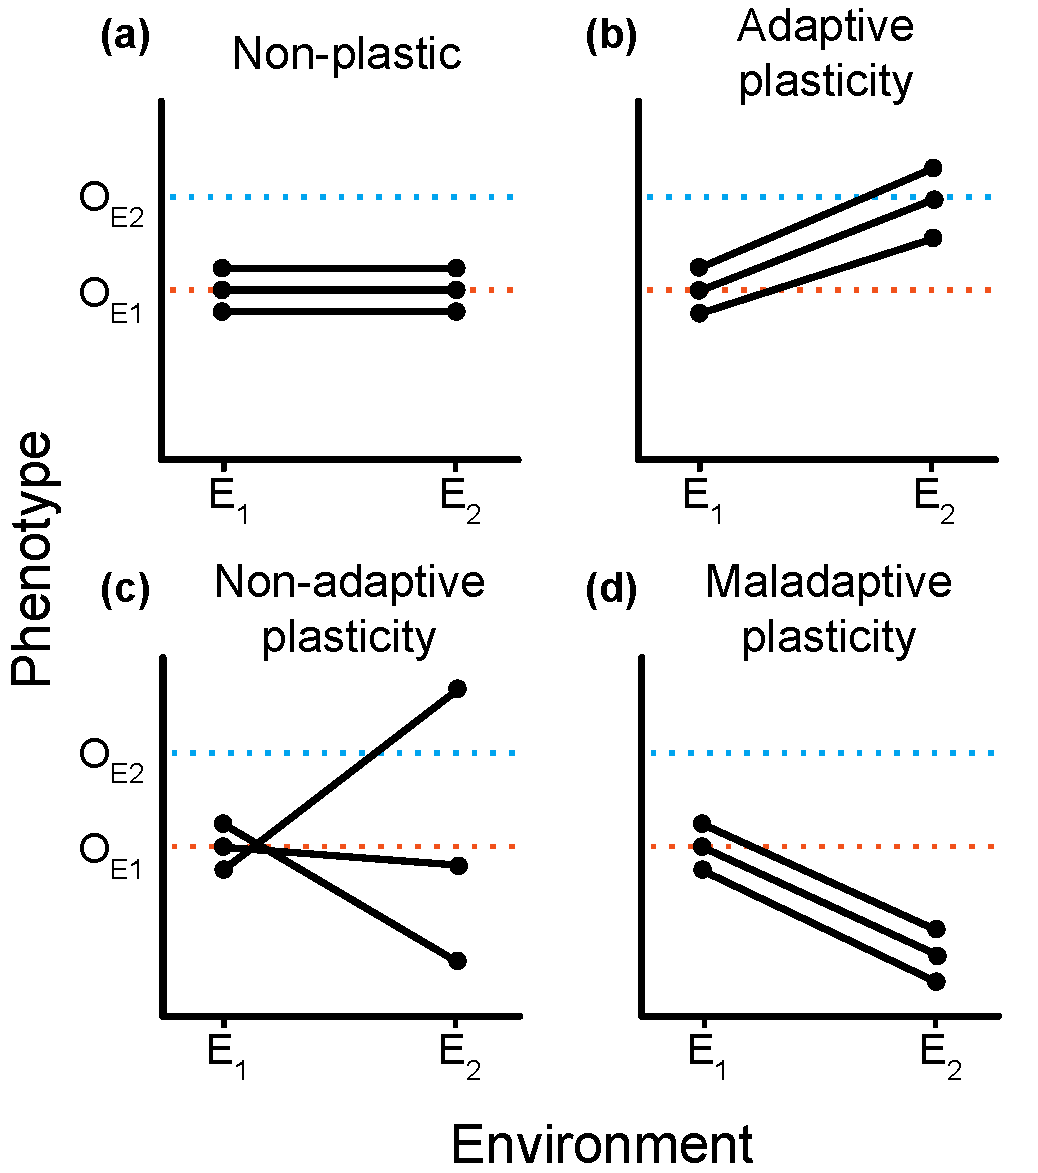
\includegraphics[width=0.65\textwidth]{media/reaction-norms.pdf}
    \caption{\small
    \textbf{Hypothetical reaction norms for genotypes placed in different environments.}
    In all panels, two environments (denoted E$_1$ and E$_2$) are shown on the x-axis.
    The y-axis indicates the phenotype expressed in each environment with O$_{\text{E}1}$ and O$_{\text{E}2}$ designating the optimal phenotype for E$_1$ and E$_2$, respectively.
    Each pair of points connected by a solid black line denotes a genotype, with the points themselves representing its hypothetical phenotypes in each environment.
    %  Each pair of points connected by a solid black line denotes a genotype, and the points represent the hypothetical phenotype expressed by organisms of that genotype within each environment.
    We present four scenarios for how populations could respond to a change from E$_1$ to E$_2$.
    (a) A non-plastic population where phenotypes do not change with environmental shifts.  In such cases, we would expect strong directional selection toward O$_{\text{E}2}$ after the environment changes.
    (b) An adaptively plastic populations where phenotypes dynamically adjust to the new optimum whenever the environment shifts. As such, we would expect this population to remain relatively stable after the environment changes.
    (c) A population exhibiting non-adaptive plasticity with substantial variation in how individuals respond to the environmental change. In this case, we expect the change in environment to result in a rapid evolutionary sweep by genotypes closest to the new optimal phenotype.
    (d) A population exhibiting maladaptive plasticity relative to the given environmental change. When the environment changes, there is little variation for selection to act on, and without beneficial mutations, this population could be at risk of extinction. 
    }
    \label{fig:reaction-norms}
\end{figure}

%%%%% OLD CAPTION

% (a) through (d) show four hypothetical reaction norm scenarios for two environments, E$_1$ (in red) to E$_2$ (in blue).  
% The optimal phenotypes for environments E$_1$ and E$_2$ are different (O$_{\text{E}1}$ and O$_{\text{E}2}$, respectively).
% In each of the four reaction norm scenarios, populations are well-adapted to E$_1$.
% In (a), genotypes in the population are non-plastic, and as such, we would expect strong directional selection on mutations that move phenotypes toward O$_{\text{E}2}$ after the environment changes.
% In (b), genotypes in the population are adaptively plastic. 
% That is, phenotypic changes induced by the environment change to E$_2$ are already near the optimum, and as such, we would expect this population to remain relatively stable after the environment changes.
% In (c), the population exhibits non-adaptive plasticity with substantial variation in how individuals respond to the environmental change. 
% In this case, we expect plasticity to result in a rapid evolutionary response to the change in environment.  
% In (d), the population exhibits maladaptive plasticity relative to the given environmental change. 
% When the environment changes, there is little variation for selection to act on, and without beneficial mutations, this population may be at risk of extinction due to their maladaptive plastic response.